\section{Methodology\label{methodology}}
% \begin{figure*}
%     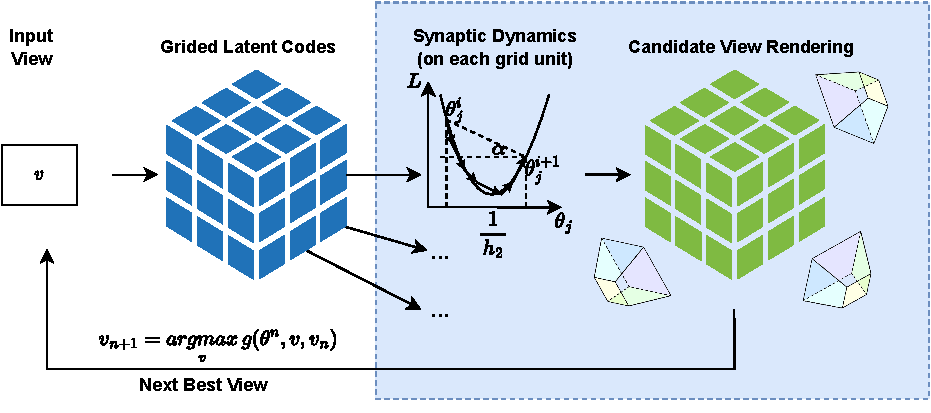
\includegraphics{overview.pdf}
%     \caption{Overview of the loss space sharpness estimation pipeline of SharpView. The left blue grid is the grid of local latent codes of grided view synthesis. The right green grid is the corresponding data grid to store the certainty estimation of each local latent codes and we directly estimate the information gain of each candidate view by directly rendering their certainty estimation in the camera frustum.}
%     \label{overview}
% \end{figure*}
Given a set of $N$ views $V=\{v_i\}_{i=1}^N$ discretized on a sphere, assume the above grided view synthesis pipeline has been trained by a subset $S\subset V$ and their corresponding groundtruth images, and the candidate views for NBV selection is $U=\frac{V}{S}$.
We approximate the information gain of a view with the value of loss function of the grided view synthesis pipeline.
To solve the NBV problem, we aim to find a view that maximize the loss between rendered image from the view and the corresponding groundtruth image, which typically complies with the sharpest loss space around the view.

\subsection{Pseudo Ray Labelling}

\begin{algorithm}[htb]
    \caption{Pseudo Ray Labelling}
    \label{alg:ray}
    \KwIn{A ray: $\bm{r}$; Set of trained views: $S$; implicit voxel grid: $G$}
    \KwOut{Pseudo accumulated rgb value of $\bm{r}$: $\hat{C}(\bm{r})$}
    \BlankLine
    
    Compute the dominant step $r^d$ along $r$;
    
    Compute the closest view $v'\in S$ from $r^d$;
    
    Cast ray $\bm{r}'$ from $v'$ to $r^d$;
    
    Render pseudo rgb value $\hat{C}(\bm{r})$ of $\bm{r}'$ from $G$.
\end{algorithm}
To compute a reasonable pseudo label for loss calculation to estimate sharpness of loss space, we use views in $S$ as references assuming that the implicit voxel grid has already fully learned knowledge from their corresponding images.
Assume we are estimating loss space sharpness of a candidate view $v$ and we are casting a ray $\bm{r}$ with $K$ steps to predict the rgb value of a pixel on the predicted image from view $v$.

In view of the continuity of rgb value when the viewing direction is slightly perturbed, a reasonable pseudo label for ray $\bm{r}$ would be the rgb value predicted from the closest trained view, which is also the most certain value that can be predicted from the grid.
As shown in Algorithm~\ref{alg:ray}, to compute the closest trained view, we first find a dominant step $r^d$ along $\bm{r}$:
\begin{equation}
    \begin{aligned}
        r^d &= r_k \\
        k & =\mathop{\arg\max}\limits_{0<i \leq K} T_i \alpha_i
    \end{aligned}
\end{equation}
$\alpha_i$ and $T_i$ are the probability of termination of ray at step $i$ and the accumulated transmittance from Equation~\ref{accu} when rendering accumulated rgb value along $\bm{r}$.
We are treating the term $T_i \alpha_i$ as weights of each step and the one with largest weight is the dominant one.

Then we cast rays from all trained views to the coordinate $x^d$ determined by $r^d$ and the ray with smallest intersection angle with $r^d$ is selected as the reference ray, and we render the rgb value $\hat{C}(\bm{r})$ of this reference ray as the pseudo label for $\bm{r}$.

\subsection{Sharpness Estimation}
The procedure of loss space sharpness estimation for a view $v$ in shown in Algorithm~\ref{alg:sharpness}.
Gathering pseudo label of each ray through each pixel on the predicted image $I$ from view $v$ we will get a pseudo image $\hat{I}$. 
After computing mean square error loss between $I$ and $\hat{I}$ and back propagating the loss, we use the norm of gradients of weights from the last layer of decoder MLP as an estimation of sharpness.
After estimating the sharpness among all candidate views in $U$, the one with highest sharpness value is selected as the next best view $v_n$.
We then acquire its groundtruth image, append to the training set $S$ and remove it from the candidate set $U$.

\begin{algorithm}[htb]
\caption{Loss Space Sharpness Estimation}
\label{alg:sharpness}
\KwIn{A candidate view: $v$; Set of trained views: $S$; implicit voxel grid: $G$; MLP decoder: $M$}
\KwOut{Sharpness of loss space around $v$: $s$}
\BlankLine
Render predicted image $I$ of $v$ with $G$ and $M$;

$\hat{I}$ = copy($I$);

\For{pixel $\in \hat{I}$}{

    Cast ray $\bm{r}$ from $v$ to pixel;

    $\hat{C}(\bm{r})$ = PseudoRayLabelling($\bm{r}$, $S$, $G$);

    Replace pixel value on $\hat{I}$ with $\hat{C}(\bm{r})$;
}

Back propagate $g_I = \frac{\partial}{\partial M_{out}} l_{mse}(I, \hat{I})$, where $M_{out}$ is the weight of the final layer;

$s$ = $\Vert g_I \Vert_2$.
\end{algorithm}
% The subtlety behind this procedure is that 

% \subsection{Next Best View}
% Given a dataset of N views discretized on a sphere $\bm{v}=\{v_i\}_{i=1}^N$, an acquisition function retrieves the groundtruth RGB image $I$ captured from a view and adds it to the training view set $S$ for training the above grided view synthesis pipeline.
% The candidate view set not yet being trained is defined as $U=\frac{\bm{v}}{\{v|v\in S\}}$.

% To solve 

